\documentclass[letterpaper, 12pt]{article}
\usepackage[letterpaper, top=2.5cm, bottom=2.5cm, left=3cm, right=3cm]{geometry} %margenes
\usepackage[utf8]{inputenc} %manejo de caracteres especiales
\usepackage[spanish]{babel} %manejo de encabezados de inglés a español
\usepackage{fancyhdr} %formato de los encabezados de página
\usepackage{ragged2e} %alineado real justficado
\usepackage{graphicx} %manejo de imagenes
\usepackage{amsmath} %manejo de notación matemática
\usepackage{mathtools} %manejo de notación matemática
\usepackage{blindtext} %texto de relleno
\usepackage{cancel} %permite la simbolización de cancelación de terminos
\usepackage{enumitem}[shortlabels] %listas con letras
\usepackage{amssymb} %manejo de simbolog►1a matematica

\pagestyle{fancy}
\fancyhf{}
\rfoot{\thepage}

\begin{document}
\setcounter{page}{1}
\thispagestyle{fancy}
\lhead{\textbf{Tarea 1, U2}}
\rhead{\textbf{14/10/2020}}
\section*{Curvas planas, ecuaciones paramétricas y coordenadas polares}
\subsection*{Convierte las coordenadas como se indica y grafica:}
\[\begin{matrix}
    \text{Rect}\rightarrow\text{Polar}& &\text{Polar}\rightarrow\text{Rect}\\
    (1,1)&&\left(3,\frac{\pi}{4}\right)\\
    (2,3)&&\left(-5,-\frac{\pi}{2}\right)\\
    (-4,5)&&\left(4,\frac{7}{4}\pi\right)
\end{matrix}\]
\subsection*{Procedimiento:}
\justify
De coordenadas rectangulares a polares:\\
\newline
(1,1):\\
\[(x,y)=(1,1),\, \text{Coord}_{\text{Polar}}=(r,\theta), \, r=\sqrt{x^2+y^2}, \, \theta=\arctan\frac{y}{x}\therefore\]
\[r=\sqrt{1^2+1^2}=\sqrt{2},\, \theta=\arctan\frac{1}{1}=\frac{\pi}{4}\therefore \text{Coord}_{\text{Polar}}=\left(\sqrt{2},\frac{\pi}{4}\right)\]
(2,3):\\
\[r=\sqrt{2^2+3^2}=\sqrt{4+9}=\sqrt{13},\,\theta=\arctan\frac{9}{4}\approx66.04\text{°}\therefore\text{Coord}_{\text{Polar}}=(\sqrt{13},66.04\text{°})\]
(-4,5):\\
\[r\sqrt{(-4)^2+5^2}=\sqrt{16+25}=\sqrt{41},\,\theta=\arctan-\frac{5}{4}\approx128.66\text{°}\therefore\text{Coord}_{\text{Polar}}=(\sqrt{41},128.66\text{°})\]
De coordenadas polares a rectangulares:\\
\newline
\(\left(3,\frac{\pi}{4}\right)\):
\\ 
\[(r,\theta)=\left(3,\frac{\pi}{4}\right),\, \text{Coord}_{\text{Rect}}=(x,y),\, x=r\cos\theta,\, y=r\sin\theta\therefore\]
\[x=3\cos\frac{\pi}{4}\approx2.12,\,y=3\sin\frac{\pi}{4}\approx 2.12\therefore(x,y)=(2.12,2.12)\]
\(\left(-5,-\frac{\pi}{2}\right)\):
\\
\[x=-5\cos-\frac{\pi}{2}=0,\,y=-5\sin-\frac{\pi}{2}=5\therefore(x,y)=(0,5)\]
\(\left(4,\frac{7}{4}\pi\right)\):
\\
\[x=4\cos\frac{7}{4}\pi\approx2.83,\,y=4\sin\frac{7}{4}\pi\approx-2.83\therefore(x,y)=(2.83,-2.83)\]
\subsection*{Gráficas: }
De coordenadas rectangulares a polares:\\
\begin{center}
    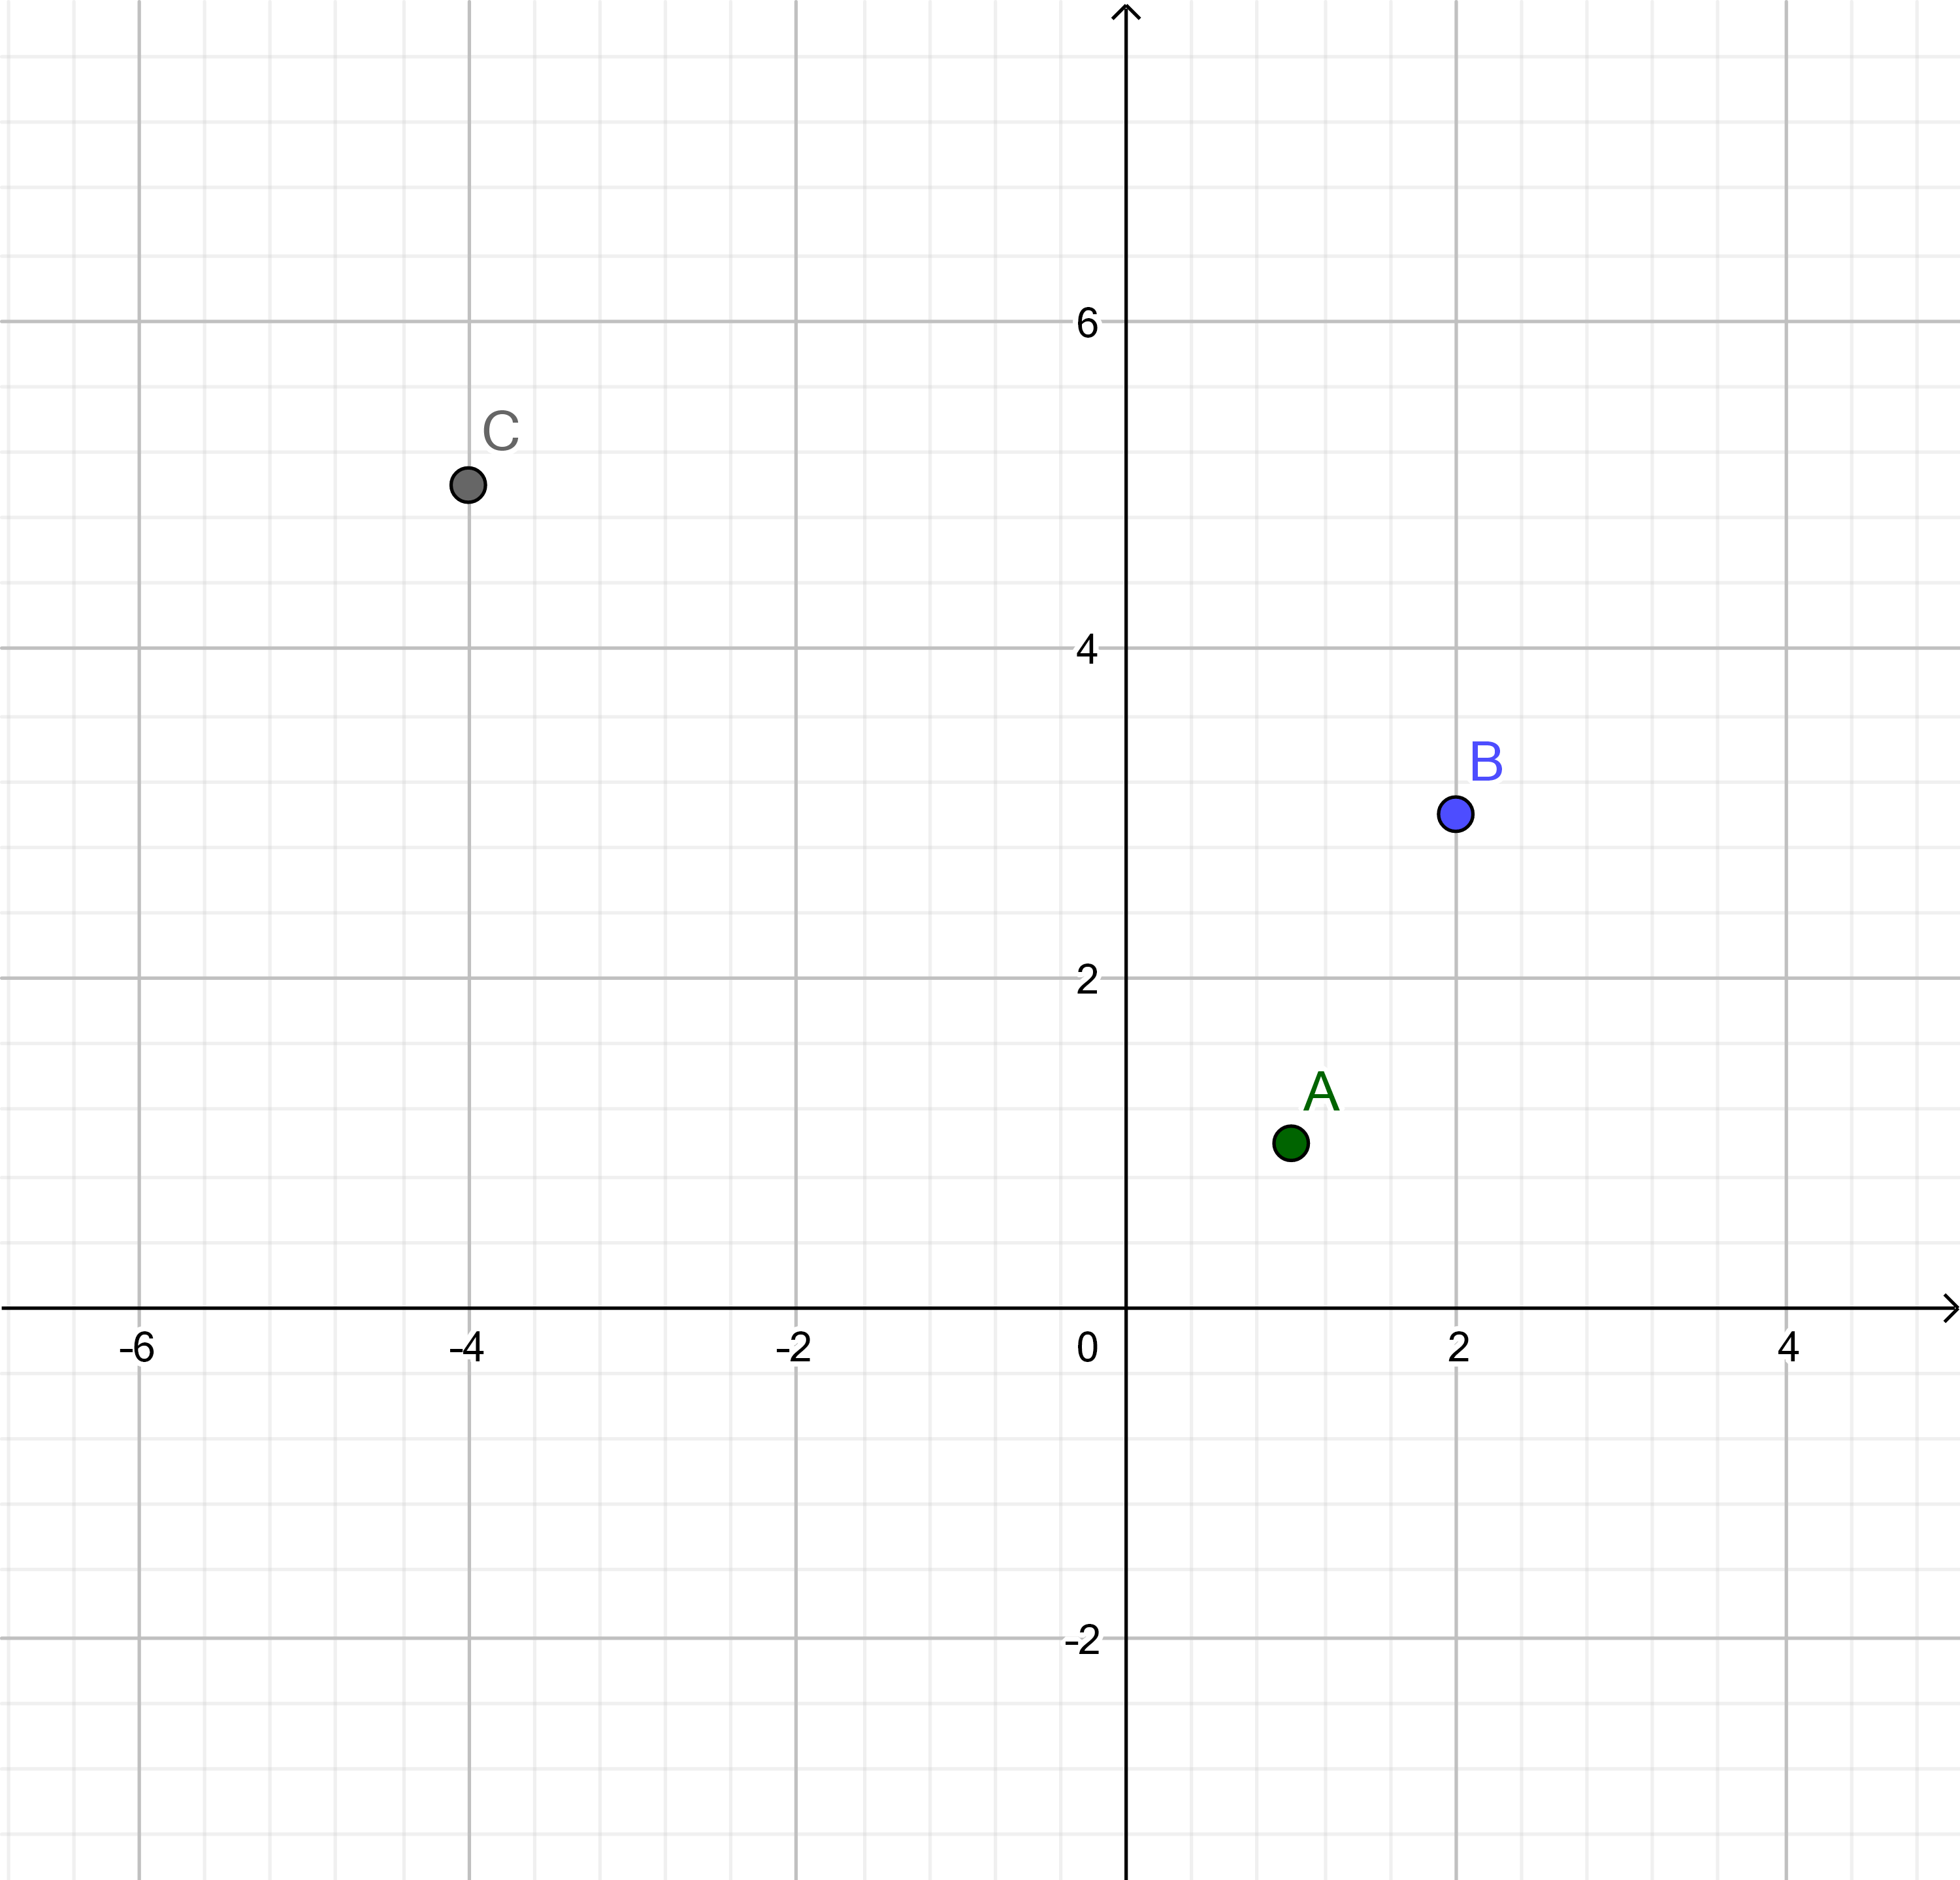
\includegraphics[width=10cm]{graph2.png}
\end{center}
De coordenadas polares a rectangulares:\\
\begin{center}
    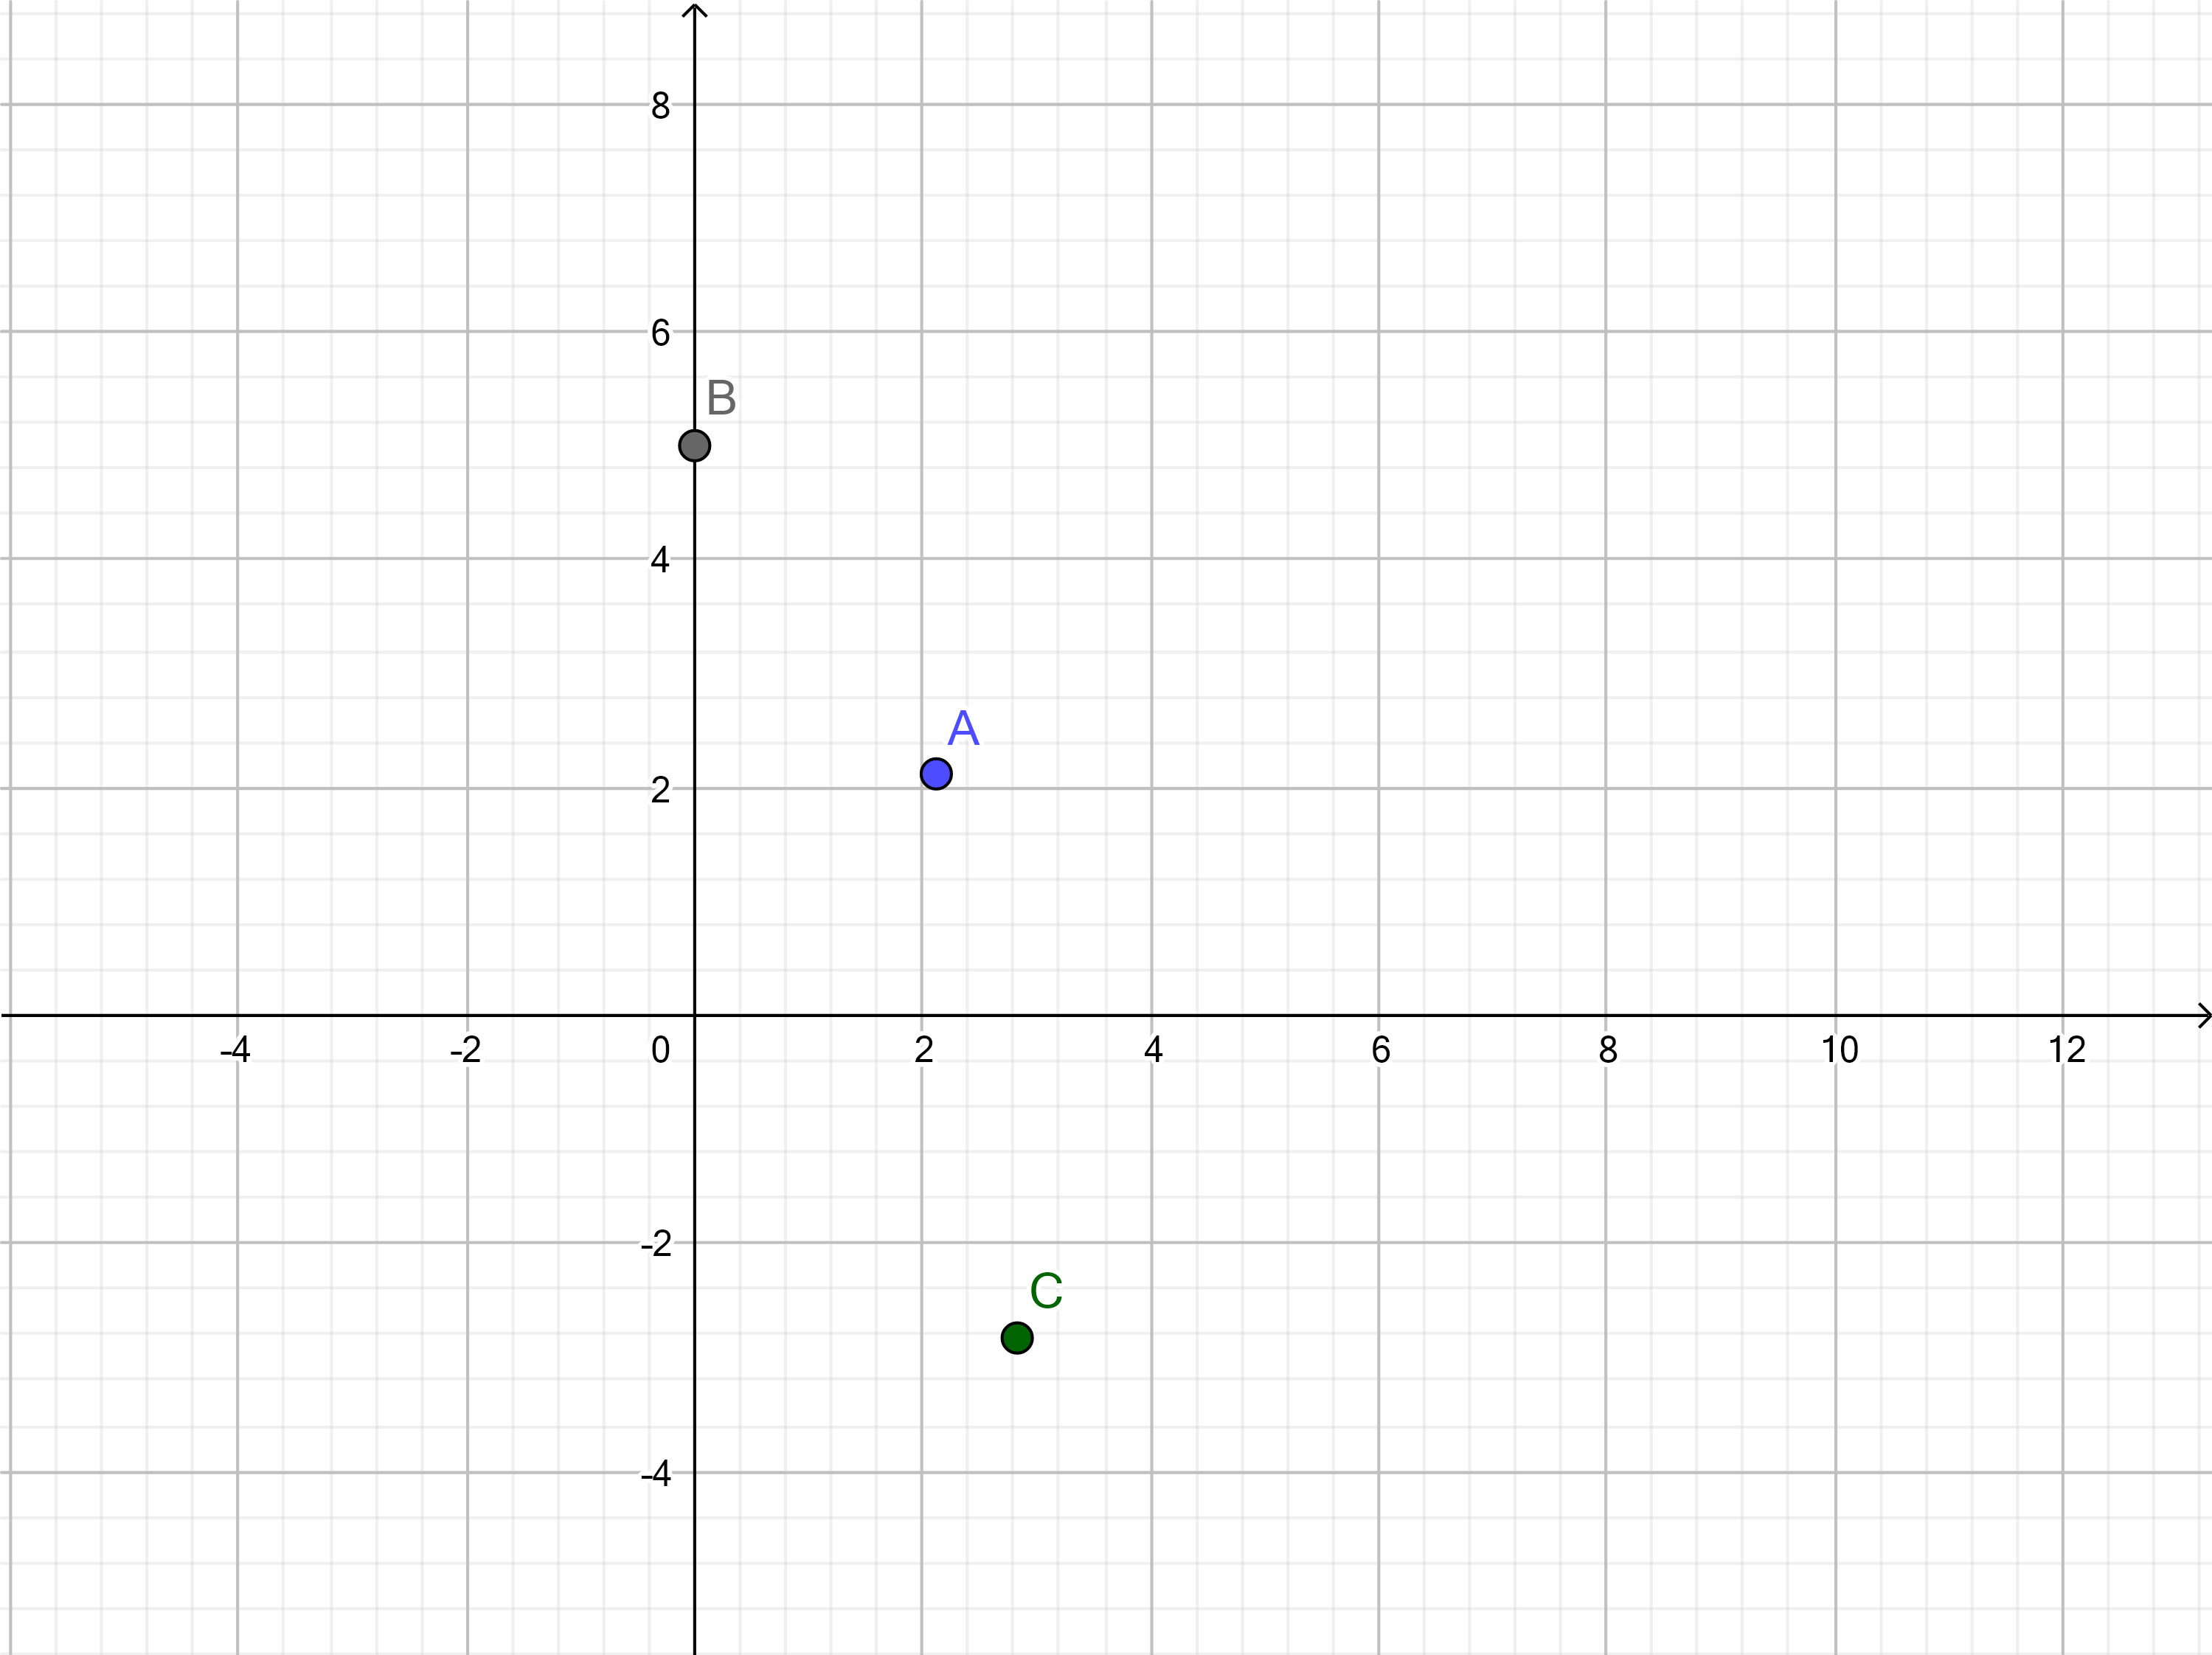
\includegraphics[width=10cm]{graph1.png}
\end{center}
\end{document}